\usepackage{pgf}
\usepackage{tikz}
\usetikzlibrary{arrows,automata,fit}

\newcommand{\ejemplografo}{
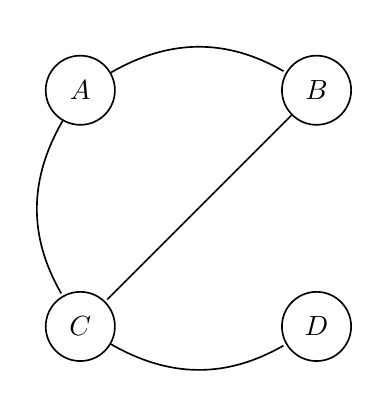
\begin{tikzpicture}[>=stealth',shorten >=1pt,auto,node distance=3cm,semithick]
  \tikzstyle{every state}=[draw=black,text=black]

  \node[state]         (A)                    {$A$};
  \node[state]         (B) [right of=A]       {$B$};
  \node[state]         (C) [below of=A]       {$C$};
  \node[state]         (D) [right of=C]       {$D$};
  
  \path (A) edge  [bend left]   node {}  (B)
            edge  [bend right]  node {}  (C)
        (B) edge                node {}  (C)
        (C) edge  [bend right]  node {}  (D);
\end{tikzpicture}}

\newcommand{\ejemplografocompleto}{
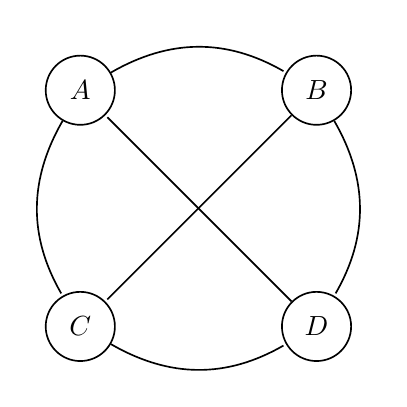
\begin{tikzpicture}[>=stealth',shorten >=1pt,auto,node distance=3cm,semithick]
  \tikzstyle{every state}=[draw=black,text=black]

  \node[state]         (A)                    {$A$};
  \node[state]         (B) [right of=A]       {$B$};
  \node[state]         (C) [below of=A]       {$C$};
  \node[state]         (D) [right of=C]       {$D$};
  
  \path (A) edge  [bend left]   node {}  (B)
            edge  [bend right]  node {}  (C)
		(B) edge  [bend left]   node {}  (D)
        (B) edge                node {}  (C)
        (D) edge                node {}  (A)
        (C) edge  [bend right]  node {}  (D);
\end{tikzpicture}}

\newcommand{\ejemplografodirigido}{
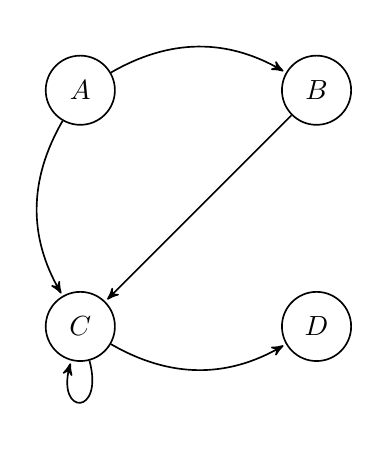
\begin{tikzpicture}[->,>=stealth',shorten >=1pt,auto,node distance=3cm,semithick]
  \tikzstyle{every state}=[draw=black,text=black]

  \node[state]         (A)                    {$A$};
  \node[state]         (B) [right of=A]       {$B$};
  \node[state]         (C) [below of=A]       {$C$};
  \node[state]         (D) [right of=C]       {$D$};
  
  \path (A) edge  [bend left]   node {}  (B)
            edge  [bend right]  node {}  (C)
        (B) edge                node {}  (C)
        (C) edge  [bend right]  node  {}  (D)
        (C) edge  [loop below]  node  {}  (C);
\end{tikzpicture}}

\newcommand{\ejemplosubgrafo}{
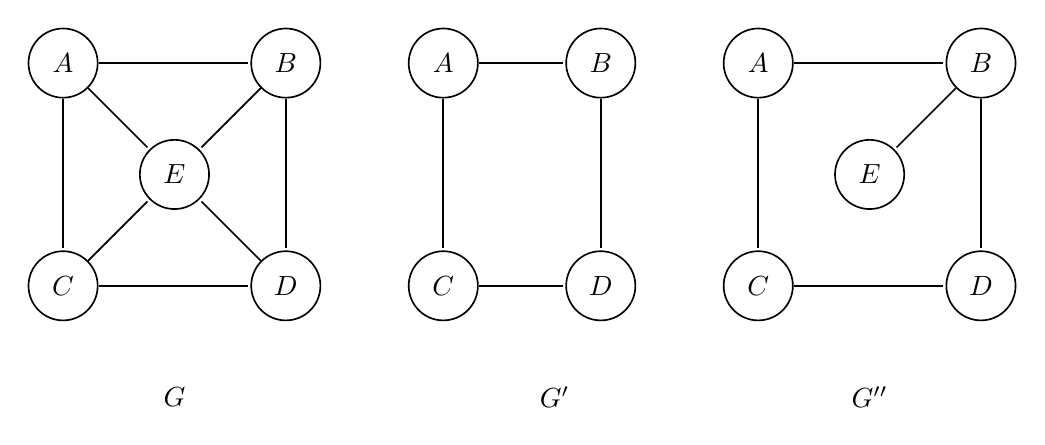
\begin{tikzpicture}[>=stealth',shorten >=1pt,auto,node distance=2cm,semithick]
  \tikzstyle{every state}=[draw=black,text=black]

% Grafo G
  \node[state]         (E)                          {$E$};
  \node[state]         (B) [above right of=E]       {$B$};
  \node[state]         (A) [above left of= E]       {$A$};
  \node[state]         (C) [below left of= E]       {$C$};
  \node[state]         (D) [below right of=E]       {$D$};

  \path (A) edge                node {}  (B)
        (A) edge                node {}  (E)
        (A) edge                node {}  (C)
        (B) edge                node {}  (D)
        (B) edge                node {}  (E)        
        (C) edge                node {}  (E)
        (C) edge                node {}  (D)
        (D) edge                node {}  (E);
        
        
% Subgrafo G'
  \node[state]         (F) [right of= B]       {$A$};
  \node[state]         (G) [right of= F]       {$B$};
  \node[state]         (H) [right of= D]       {$C$};
  \node[state]         (I) [right of= H]       {$D$};
  
  \path (F) edge                node {}  (G)
        (F) edge                node {}  (H)
        (G) edge                node {}  (I)
        (H) edge                node {}  (I);
        
% Subgrafo G'

  \node[state]         (J) [right of= G]             {$A$};
  \node[state]         (K) [right of= I]             {$C$};
  \node[state]         (N) [above right of= K]       {$E$};
  \node[state]         (M) [below right of= N]       {$D$};
  \node[state]         (L) [above right of= N]       {$B$};
  
  \path (J) edge                node {}  (K)
        (J) edge                node {}  (L)
        (L) edge                node {}  (N)
        (L) edge                node {}  (M)
        (K) edge                node {}  (M);
        
% Etiquetas con el nombre de los grafos
  \node[align=center, below right of=C] {$G$};
  \node[align=center, below right of=H] {$G'$};
  \node[align=center, below right of=K] {$G''$};
\end{tikzpicture}}

\newcommand{\ejemplounionintersecciongrafo}{
\begin{tikzpicture}[>=stealth',shorten >=1pt,auto,node distance=2cm,semithick]
  \tikzstyle{every state}=[draw=black,text=black]

% Grafo G
  \node[state]         (A)                          {$A$};
  \node[state]         (B) [below right of=A]       {$B$};
  \node[state]         (C) [below      of= B]       {$C$};
  \node[state]         (D) [right of=B]             {$D$};
  \node[state]         (E) [right of=C]             {$E$};

  \path (A) edge                node {}  (B)
        (B) edge                node {}  (C)
        (B) edge                node {}  (D)      
        (C) edge                node {}  (E)
        (D) edge                node {}  (E);
        
% Grafo G'
  \node[state]         (H) [right of= E]       {$C$};
  \node[state]         (I) [right of= D]       {$D$};
  \node[state]         (G) [right of= H]       {$E$};
  \node[state]         (F) [above right of= G] {$F$};
  
  \path (H) edge                node {}  (I)
        (I) edge                node {}  (F)
        (G) edge                node {}  (F)
        (H) edge                node {}  (G);
        
% Etiquetas con el nombre de los grafos
  \node[align=center, below right of=C] (Z) {$G$};
  \node[align=center, below right of=H] (Y) {$G'$};

% Grafo G \cup G'
  \node[state]         (J) [below left of=Z]        {$A$};
  \node[state]         (K) [below right of=J]       {$B$};
  \node[state]         (L) [below of= K]            {$C$};
  \node[state]         (M) [right of=K]             {$D$};
  \node[state]         (N) [right of=L]             {$E$};
  \node[state]         (R) [above right of=N]       {$F$};

  \path (J) edge                node {}  (K)
        (K) edge                node {}  (L)
        (K) edge                node {}  (M)      
        (L) edge                node {}  (N)
        (L) edge                node {}  (M)
        (N) edge                node {}  (R)
        (R) edge                node {}  (M)
        (M) edge                node {}  (N);
        
  \node[align=center, below right of=L] {$G \cup G'$};
  
% Grafo G \cup G'
  \node[state]         (O) [right of=R]        {$C$};
  \node[state]         (P) [right of=O]              {$E$};


  \path (O) edge                node {}  (P);
        
        
  \node[align=center, below right of=O] {$G \cap G'$};

\end{tikzpicture}}


\newcommand{\ejemplomarkov}{
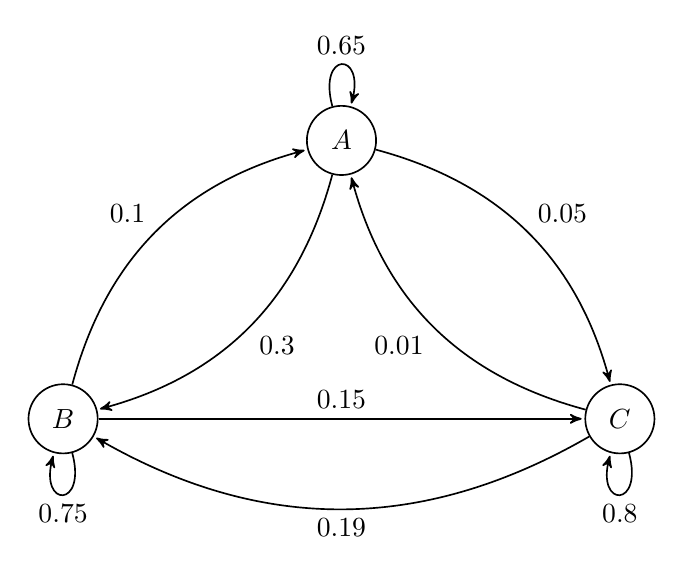
\begin{tikzpicture}[->,>=stealth',shorten >=1pt,auto,node distance=5cm,semithick]
  \tikzstyle{every state}=[draw=black,text=black]

  \node[state]         (A)                    {$A$};
  \node[state]         (B) [below left of=A]  {$B$};
  \node[state]         (C) [below right of=A] {$C$};
  
  \path (A) edge  [loop above] node {$0.65$} (A)
            edge  [bend left]  node {$0.3$}  (B)
            edge  [bend left]  node {$0.05$} (C)
        (B) edge  [loop below] node {$0.75$} (B)
            edge  [bend left]  node {$0.1$}  (A)
            edge               node {$0.15$} (C)
        (C) edge  [loop below] node {$0.8$}  (C)
            edge  [bend left]  node {$0.01$} (A)
            edge  [bend left]  node {$0.19$} (B);
\end{tikzpicture}}

\newcommand{\ejemplomarkovcompleto}{
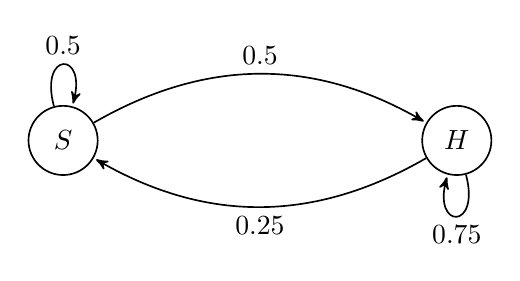
\begin{tikzpicture}[->,>=stealth',shorten >=1pt,auto,node distance=5cm,semithick]
  \tikzstyle{every state}=[draw=black,text=black]

  \node[state]         (S)                    {$S$};
  \node[state]         (H)      [right of=S]  {$H$};
  
  \path (S) edge  [loop above] node {$0.5$}  (S)
            edge  [bend left]  node {$0.5$}  (H)
        (H) edge  [loop below] node {$0.75$} (H)
            edge  [bend left]  node {$0.25$} (S);

\end{tikzpicture}}

\newcommand{\ejemplografomarkov}{
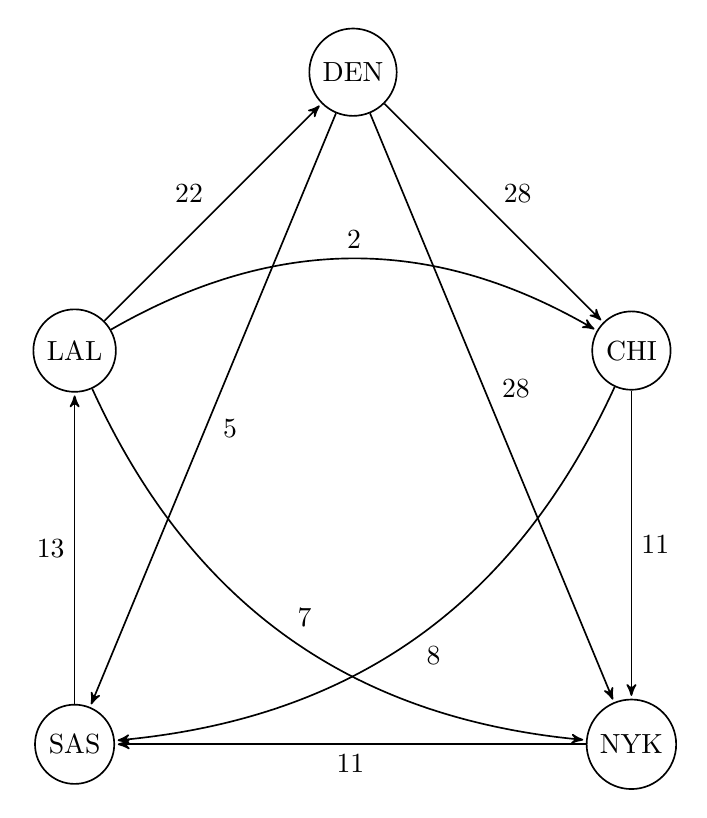
\begin{tikzpicture}[->,>=stealth',shorten >=1pt,auto,node distance=5cm,semithick]
  \tikzstyle{every state}=[draw=black,text=black]

  \node[state]         (A)                         {DEN};
  \node[state]         (B)      [below left of=A]  {LAL};
  \node[state]         (C)      [below of=B]       {SAS};
  \node[state]         (D)      [below right of=A] {CHI};
  \node[state]         (E)      [below of=D]       {NYK};
  
  \path (A) edge                node {$5$}   (C)
            edge                node {$28$}  (D)
            edge                node {$28$}  (E)
        (B) edge                node {$22$}  (A)
	        edge [bend right]   node {$7$}   (E)
            edge [bend left]    node {$2$}   (D)
        (C) edge                node {$13$}  (B)
	    (D) edge [bend left]    node {$8$}   (C)
            edge                node {$11$}  (E)
        (E) edge                node {$11$}  (C);
        	
\end{tikzpicture}}

\newcommand{\ejemplografomassey}{
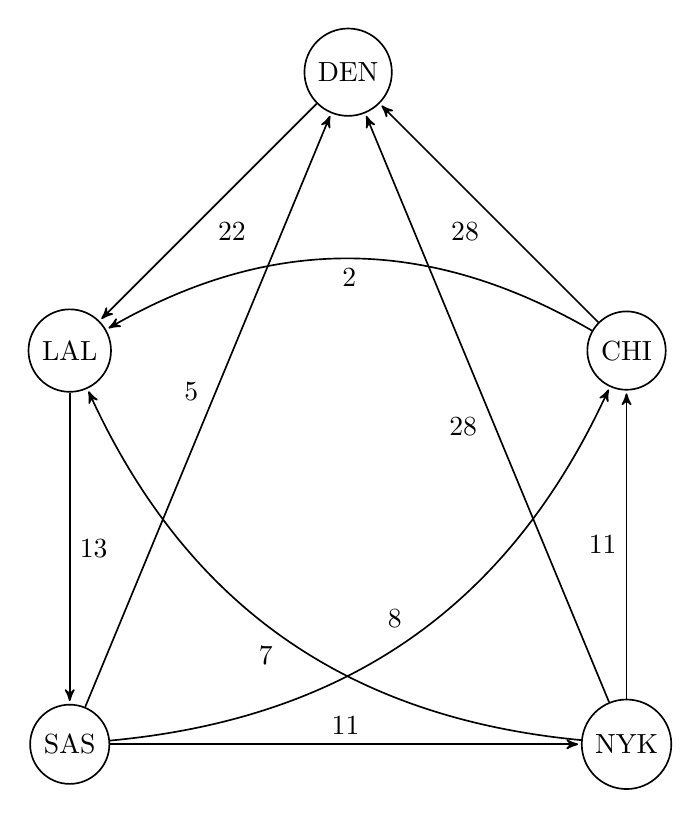
\begin{tikzpicture}[->,>=stealth',shorten >=1pt,auto,node distance=5cm,semithick]
  \tikzstyle{every state}=[draw=black,text=black]

  \node[state]         (A)                         {DEN};
  \node[state]         (B)      [below left of=A]  {LAL};
  \node[state]         (C)      [below of=B]       {SAS};
  \node[state]         (D)      [below right of=A] {CHI};
  \node[state]         (E)      [below of=D]       {NYK};
  
  \path (C) edge   node {$5$}   (A)
        (D) edge   node {$28$}  (A)
        (E) edge   node {$28$}  (A)
        (A) edge   node {$22$}  (B)
	    (E) edge [bend left]  node {$7$}   (B)
        (D) edge [bend right]  node {$2$}   (B)
        (B) edge   node {$13$}  (C)
	    (C) edge [bend right]  node {$8$}   (D)
        (E) edge   node {$11$}  (D)
        (C) edge   node {$11$}  (E);
        	
\end{tikzpicture}}

\newcommand{\agregacionrankings}{
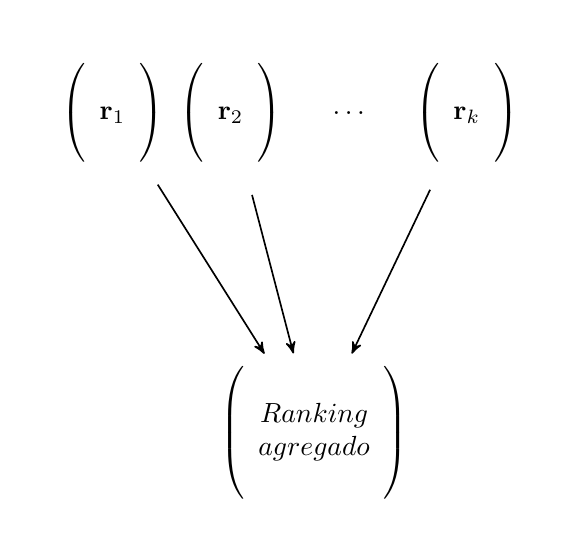
\begin{tikzpicture}[->,>=stealth',shorten >=1pt,auto,node distance=1.5cm,semithick]
  \tikzstyle{every state}=[draw opacity=0,draw=white,text=black]

  \node[state]         (A)                         {$\left(\begin{array}{c}
\ \\
\mathbf{r}_1 \\
\ \\
  \end{array}\right)$};
  \node[state]         (B)      [right of=A]  {$\left(\begin{array}{c}
\ \\
\mathbf{r}_2 \\
\ \\
  \end{array}\right)$};
  \node[state]         (C)      [right of=B]       {$\dots$};
  \node[state]         (D)      [right of=C] {$\left(\begin{array}{c}
  \ \\
  \mathbf{r}_k \\
  \ \\
    \end{array}\right)$};
\node[state]         (E)      [below right of=B] {};
\node[state]         (G)      [below       of=E] {};
\node                (F)      [below of=G]       {$\left(\begin{array}{c}
  \ \\
  \text{Ranking} \\
  \text{agregado} \\
  \ \\
    \end{array}\right)$};
    
  
  \path (A) edge   node {}   (F)
        (B) edge   node {}   (F)
        (D) edge   node {}   (F);
        	
\end{tikzpicture}}

\newcommand{\partidossimulados}{
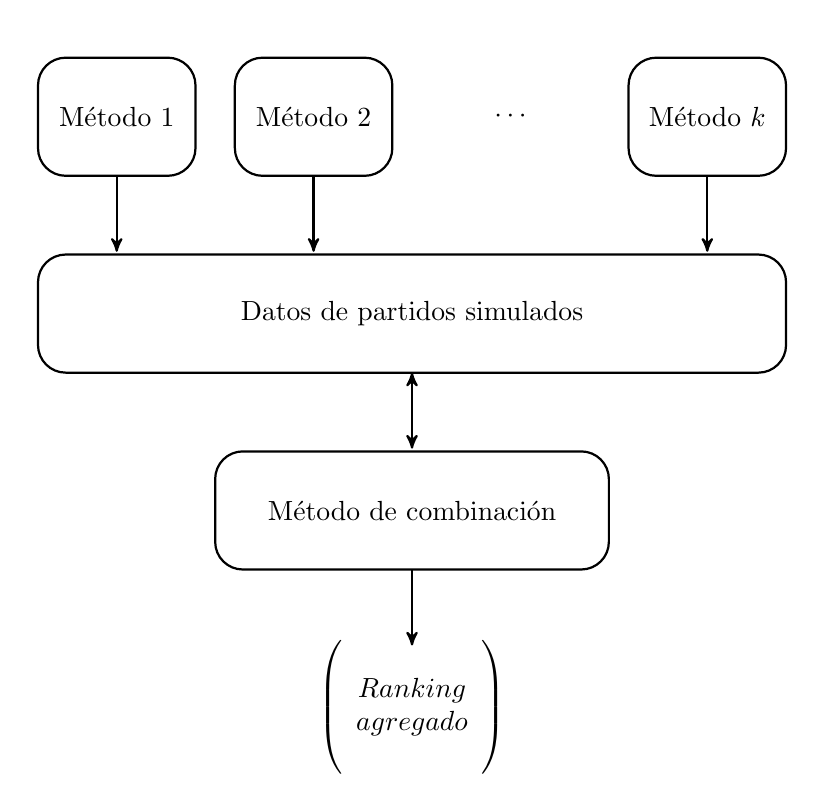
\begin{tikzpicture}[->,>=stealth',shorten >=1pt,auto,node distance=2.5cm,semithick]
  \tikzstyle{every state}=[draw=white,text=black]
	\node         (A) [draw,thick,minimum width=2cm,minimum height=1.5cm,rounded corners=10pt] {Método $1$};
	  
    \node         (B) [draw,thick,minimum width=2cm,minimum height=1.5cm, right of=A,rounded corners=10pt] {Método $2$};

   \node[state]         (C) [draw,thick,minimum width=2cm,minimum height=1.5cm, right of=B, rounded corners=10pt] {$\cdots$};

   \node         (D) [draw,thick,minimum width=2cm,minimum height=1.5cm, right of=C, rounded corners=10pt] {Método $k$};

   \node[fit=(A)(B)(C)(D)](group){};
	  
   \node         (E) [draw,thick,minimum width=9.5cm,minimum height=1.5cm, below of=group, rounded corners=10pt] {Datos de partidos simulados};
   
   \node         (F) [draw,thick,minimum width=5cm,minimum height=1.5cm, below of=E, rounded corners=10pt] {Método de combinación};
   
   \node         (G) [thick,minimum width=5cm,minimum height=1.5cm, below of=F, rounded corners=10pt] {$\left(\begin{array}{c}
   \\ 
   \text{Ranking}\\
   \text{agregado}\\
   \\
   \end{array}\right)$};
   
  
  \draw[->, thick] (0,-0.75) to (0,-1.75);
  \draw[->, thick] (2.5,-0.75) to (2.5,-1.75);
  \draw[->, thick] (7.5,-0.75) to (7.5,-1.75);
  \draw[<->, thick] (3.75,-3.25) to (3.75,-4.25);
  \draw[->, thick] (3.75,-5.75) to (3.75,-6.75);
       
\end{tikzpicture}}

\newcommand{\ejemploregionfactible}{
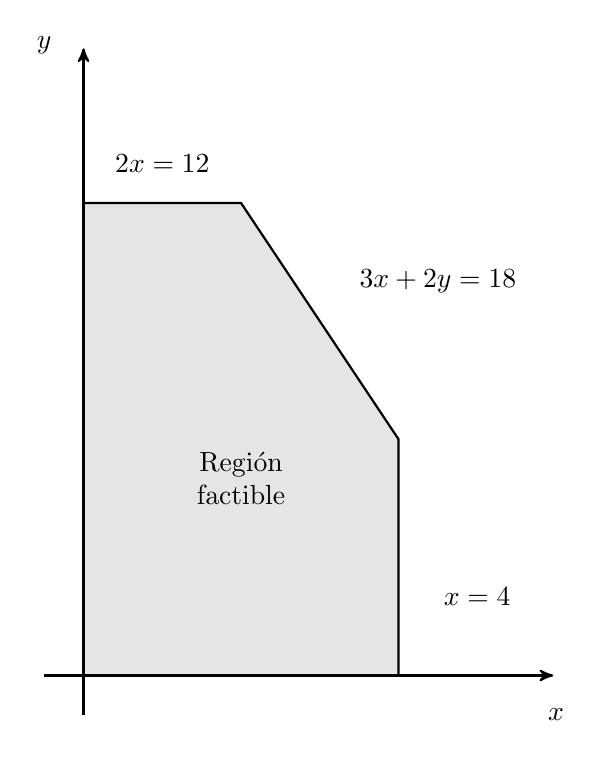
\begin{tikzpicture}[->,>=stealth',shorten >=1pt,auto,node distance=2.5cm,semithick]
  \tikzstyle{every state}=[draw=white,text=black]
 
  % Región factible
  \draw[thick, fill=gray!20] (0,0) -- (0,6) -- (2,6) -- (4,3) -- (4,0) -- cycle;
  \node[align=center] at (2,2.5) (factible) {Región \\ factible};

  % Ejes
  \draw[->, thick] (-0.5,0) to (6,0);
  \draw[->, thick] (0,-0.5) to (0,8);
  \node[align=center] at (6,-0.5) {$x$};
  \node[align=center] at (-0.5,8) {$y$};
  
  % Restricciones
  \node[align=center] (r1) at (1,6.5) {$2x = 12$};
  \node[align=center] (r2) at (4.5,5) {$3x + 2y = 18$};
  \node[align=center] (r3) at (5,1) {$x = 4$};
\end{tikzpicture}}

\newcommand{\ejemplografodominancia}{
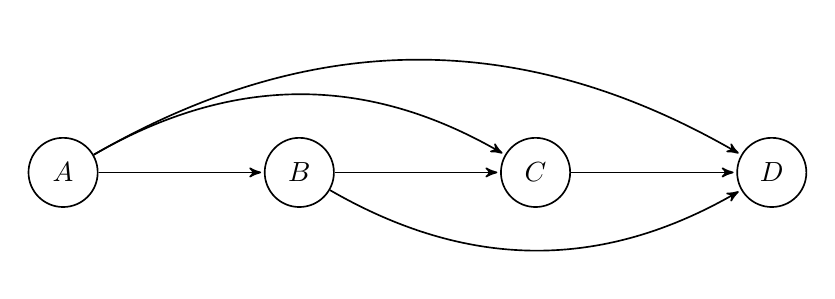
\begin{tikzpicture}[->,>=stealth',shorten >=1pt,auto,node distance=3cm,semithick]
  \tikzstyle{every state}=[draw=black,text=black]
 
  
  \node[state] (A)              {$A$};
  \node[state] (B) [right of=A] {$B$};
  \node[state] (C) [right of=B] {$C$};
  \node[state] (D) [right of=C] {$D$};
  
  \path (A) edge              node {} (B);
  \path (A) edge [bend left]  node {} (C);
  \path (A) edge [bend left]  node {} (D);
  \path (B) edge              node {} (C);
  \path (B) edge [bend right] node {} (D);
  \path (C) edge              node {} (D);
  
\end{tikzpicture}}

\newcommand{\ejemplografodominanciaoptimo}{
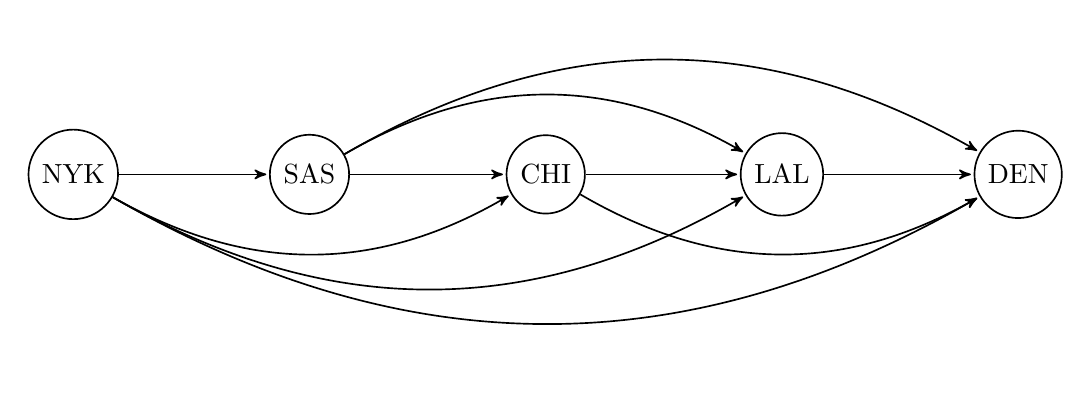
\begin{tikzpicture}[->,>=stealth',shorten >=1pt,auto,node distance=3cm,semithick]
  \tikzstyle{every state}=[draw=black,text=black]
 
  
  \node[state] (nyk)                {NYK};
  \node[state] (sas) [right of=nyk] {SAS};
  \node[state] (chi) [right of=sas] {CHI};
  \node[state] (lal) [right of=chi] {LAL};
  \node[state] (den) [right of=lal] {DEN};  
  
  \path (nyk)   edge [bend right]  node {} (chi);
  \path (nyk)   edge [bend right]  node {} (lal);
  \path (nyk)   edge [bend right]  node {} (den);
  \path (nyk)   edge               node {} (sas);
  \path (sas)   edge [bend left]   node {} (lal);
  \path (sas)   edge [bend left]   node {} (den);  
  \path (sas)   edge               node {} (chi);
  \path (chi)   edge               node {} (lal);
  \path (chi)   edge [bend right]  node {} (den);    
  \path (lal)   edge               node {} (den);

\end{tikzpicture}}

\newcommand{\ejemplografocompetitividad}{
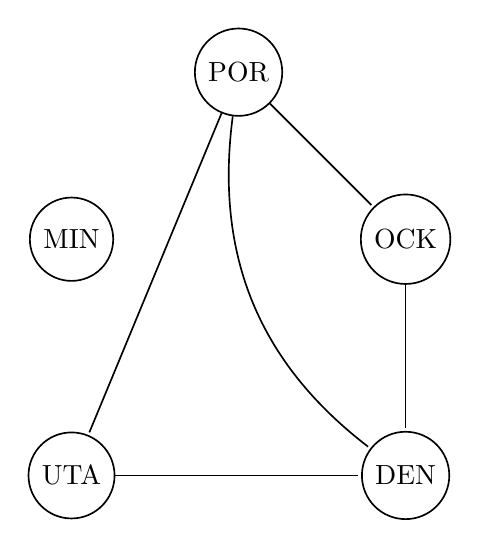
\begin{tikzpicture}[>=stealth',shorten >=1pt,auto,node distance=3cm,semithick]
  \tikzstyle{every state}=[draw=black,text=black]
 
  
  \node[state] (por)                      {POR};
  \node[state] (ock) [below right of=por] {OCK};
  \node[state] (den) [below       of=ock] {DEN};
  \node[state] (min) [below left  of=por] {MIN};
  \node[state] (uta) [below       of=min] {UTA};  
  
  \path (por)   edge                node {} (ock);
  \path (por)   edge [bend right]   node {} (den);  
  \path (por)   edge                node {} (uta);
  \path (uta)   edge                node {} (den);
  \path (ock)   edge                node {} (den);
  
\end{tikzpicture}}

\newcommand{\ejemplografoponderado}{
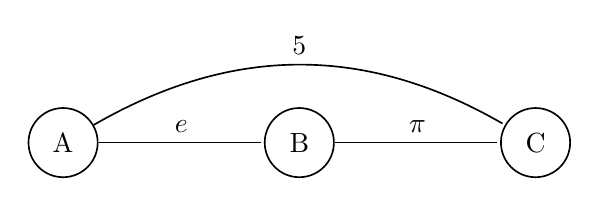
\begin{tikzpicture}[>=stealth',shorten >=1pt,auto,node distance=3cm,semithick]
  \tikzstyle{every state}=[draw=black,text=black]
 
  
  \node[state] (a)              {A};
  \node[state] (b) [right of=a] {B};
  \node[state] (c) [right of=b] {C};
  
  \path (a)     edge                node {$e$} (b);
  \path (a)   edge [bend left]   node {$5$} (c);  
  \path (b)   edge                node {$\pi$} (c);
 
  
\end{tikzpicture}}

\newcommand{\ejemplografocompetitividadevolutivo}{
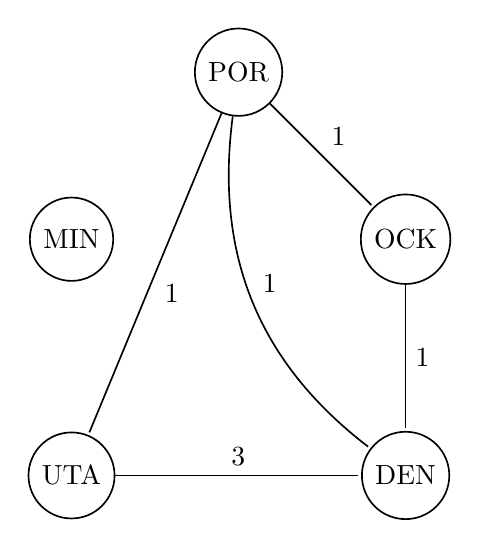
\begin{tikzpicture}[>=stealth',shorten >=1pt,auto,node distance=3cm,semithick]
  \tikzstyle{every state}=[draw=black,text=black]
 
  
  \node[state] (por)                      {POR};
  \node[state] (ock) [below right of=por] {OCK};
  \node[state] (den) [below       of=ock] {DEN};
  \node[state] (min) [below left  of=por] {MIN};
  \node[state] (uta) [below       of=min] {UTA};  
  
  \path (por)   edge                node {$1$} (ock);
  \path (por)   edge [bend right]   node {$1$} (den);  
  \path (por)   edge                node {$1$} (uta);
  \path (uta)   edge                node {$3$} (den);
  \path (ock)   edge                node {$1$} (den);
  
\end{tikzpicture}}

\newcommand{\ejemplogradomedio}{
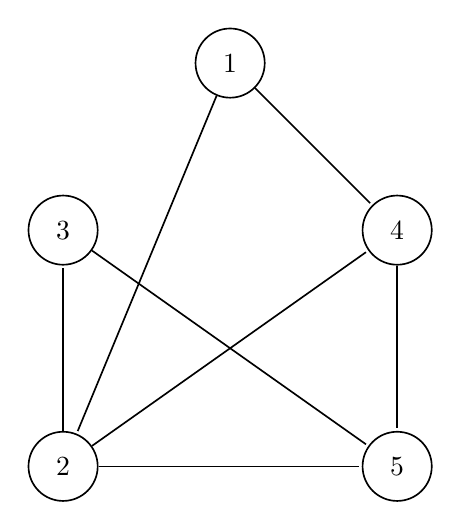
\begin{tikzpicture}[>=stealth',shorten >=1pt,auto,node distance=3cm,semithick]
  \tikzstyle{every state}=[draw=black,text=black]
 
  
  \node[state] (1)                      {1};
  \node[state] (4) [below right of=1] {4};
  \node[state] (5) [below       of=4] {5};
  \node[state] (3) [below left  of=1] {3};
  \node[state] (2) [below       of=3] {2};  
  
  \path (1)   edge                node {} (4);
  \path (1)   edge                node {} (2);  
  \path (2)   edge                node {} (4);
  \path (2)   edge                node {} (5);
  \path (2)   edge                node {} (3);
  \path (4)   edge                node {} (5); 
  \path (3)   edge                node {} (5); 
  
\end{tikzpicture}}

\newcommand{\ejemplofuerzamedia}{
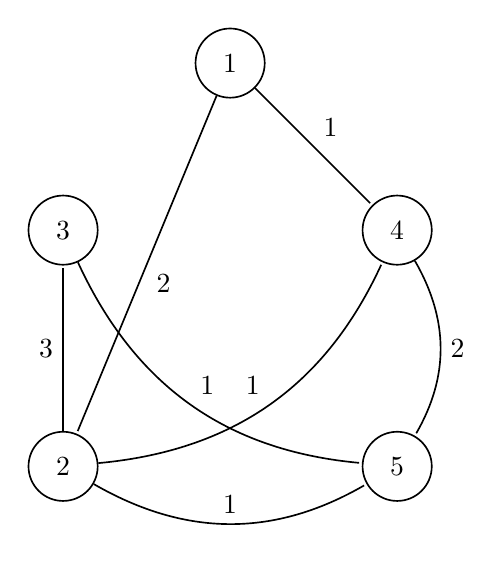
\begin{tikzpicture}[>=stealth',shorten >=1pt,auto,node distance=3cm,semithick]
  \tikzstyle{every state}=[draw=black,text=black]
 
  
  \node[state] (1)                      {1};
  \node[state] (4) [below right of=1] {4};
  \node[state] (5) [below       of=4] {5};
  \node[state] (3) [below left  of=1] {3};
  \node[state] (2) [below       of=3] {2};  
  
  \path (1)   edge                node {$1$} (4);
  \path (1)   edge    node {$2$} (2);  
  \path (2)   edge   [bend right]  node {$1$} (4);
  \path (2)   edge   [bend right] node {$1$} (5);
  \path (2)   edge                node {$3$} (3);
  \path (4)   edge   [bend left]  node {$2$} (5); 
  \path (3)   edge   [bend right]  node {$1$} (5); 
  
\end{tikzpicture}}

\newcommand{\ejemplografocordal}{\begin{tikzpicture}[>=stealth',shorten >=1pt,auto,node distance=3cm,semithick]
  \tikzstyle{every state}=[draw=black,text=black]
 
  \node[state] (1)                      {1};
  \node[state] (4) [below right of=1]   {4};
  \node[state] (2) [below left  of=1]   {2};
  \node[state] (3) [below left  of=4]   {3};
  \node[state] (5) [right       of=4]   {5};  
  \node[state] (6) [right       of=5]   {6};    
  
  \path (1)   edge    node {} (4);
  \path (1)   edge    node {} (2);  
  \path (1)   edge    node {} (3); 
  \path (2)   edge    node {} (4);   
  \path (2)   edge    node {} (3);
  \path (3)   edge    node {} (4);
  \path (4)   edge    node {} (5);
  \path (5)   edge    node {} (6);            
  
\end{tikzpicture}}

\newcommand{\ejemplografopermutacion}{
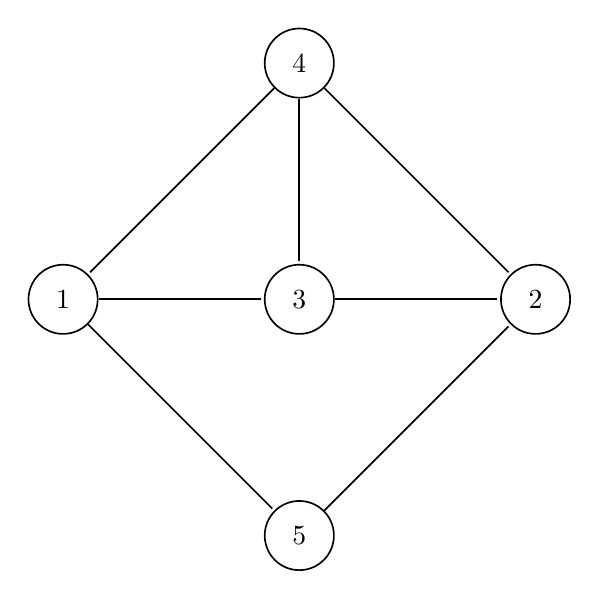
\begin{tikzpicture}[>=stealth',shorten >=1pt,auto,node distance=3cm,semithick]
  \tikzstyle{every state}=[draw=black,text=black]
 
  \node[state] (1)                      {4};
  \node[state] (4) [below       of=1]   {3};
  \node[state] (2) [left  of=4]         {1};
  \node[state] (3) [below       of=4]   {5};
  \node[state] (5) [right       of=4]   {2};  
  
  \path (1)   edge    node {} (4);
  \path (1)   edge    node {} (2);  
  \path (2)   edge    node {} (4); 
  \path (2)   edge    node {} (3);
  \path (3)   edge    node {} (5);
  \path (1)   edge    node {} (5);
  \path (4)   edge    node {} (5);
  
\end{tikzpicture}}

\newcommand{\ejemplografocomparabilidad}{
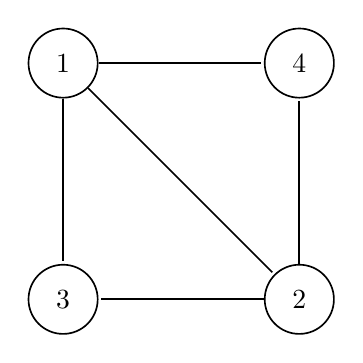
\begin{tikzpicture}[>=stealth',shorten >=1pt,auto,node distance=3cm,semithick]
  \tikzstyle{every state}=[draw=black,text=black]
 
  \node[state] (1)                      {1};
  \node[state] (4) [below       of=1]   {3};
  \node[state] (2) [right  of=4]         {2};
  \node[state] (3) [right       of=1]   {4};
  
  
  \path (1)   edge    node {} (4);
  \path (1)   edge    node {} (2);  
  \path (2)   edge    node {} (4); 
  \path (2)   edge    node {} (3);
  \path (1)   edge    node {} (3);
  
\end{tikzpicture}}

\newcommand{\ejemplogfgrafo}{
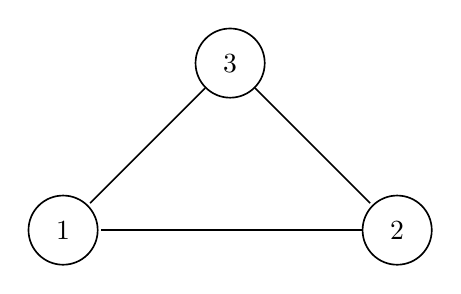
\begin{tikzpicture}[>=stealth',shorten >=1pt,auto,node distance=3cm,semithick]
  \tikzstyle{every state}=[draw=black,text=black]
 
  \node[state] (1)                    {3};
  \node[state] (4) [below left  of=1] {1};
  \node[state] (2) [below right of=1] {2};
  
  \path (1)   edge    node {} (4);
  \path (1)   edge    node {} (2);  
  \path (2)   edge    node {} (4); 
  
\end{tikzpicture}}